% !TEX root = Slide_HUST.tex
\documentclass[t, aspectratio=169]{beamer} % Khai báo tỉ lệ cho Beamer biết
\usepackage[utf8]{vietnam}
\usepackage{amsthm,amsmath,amssymb}
\usepackage{lmodern}
\usepackage{graphicx}
%\usepackage{times} % Đổi font chữ sang Times New Roman (không khuyến khích vì font xấu quá)

% --- CẤU HÌNH LỀ (Phải đặt ở đây) ---
\def\slideContentLeftMargin{0.5cm}  % Lề trái
\def\slideContentRightMargin{1cm}   % Lề phải
\def\hustHeaderHeight{1cm}        % Lề trên (Né thanh tiêu đề)
\def\slideContentBotMargin{3.5cm}   % Lề dưới (Né logo/footer)


% Thay đổi [red] thành [blue] để đổi màu
% Thay đổi [169] thành [43] (nhớ đổi cả trong documentclass) để đổi tỉ lệ
\usepackage[blue, 169]{beamerthemeHUST}
\usetikzlibrary{arrows.meta,calc} 

% 1. Điều chỉnh vị trí cả khối title ở trang title
\renewcommand{\titlePageTitleX}{-0.5cm}
\renewcommand{\titlePageTitleY}{-0.5cm}

% Cỡ chữ tiêu đề
\renewcommand{\hustTitleFontSize}{\huge}

% 2. Căn lề TỪNG THÀNH PHẦN của trang title
% - Tiêu đề chính: Căn TRÁI
\renewcommand{\hustTitleAlign}{\alignLeft} 

% - Phụ đề: Căn TRÁI
\renewcommand{\hustSubtitleAlign}{\alignLeft}

% - Tác giả & Trường: Căn TRÁI
\renewcommand{\hustAuthorAlign}{\alignLeft}
\renewcommand{\hustInstAlign}{\alignLeft}


% Bạn có thể dùng \\ để xuống dòng thủ công trong phần title
\title{HIỂN THỊ GIAO THÔNG TRONG KHÔNG GIAN 3D \\ TỪ DỮ LIỆU MÔ PHỎNG SUMO}
\subtitle{Báo cáo Đồ án tốt nghiệp}
\author{\texorpdfstring{Đặng Minh Hoàng -- 20225719}{Đặng Minh Hoàng -- 20225719}}
\institute{Chương trình: Công nghệ thông tin Việt-Nhật }
\date{Hà Nội, 06/2026}

\begin{document}
	
	\hustintropage{} % Có thể comment trang này để tắt slide đi, nếu không muốn sử dụng.
	%\hustsectionpage{} % Có thể comment trang này để tắt slide đi, nếu không muốn sử dụng.
	
	
	
	
	% Trang bìa
	\husttitlepage
	
	\begin{frame}[allowframebreaks]{Nội dung trình bày}
		\tableofcontents %Mục lục slide, sử dụng \tableofcontents[hideallsubsections] nếu mục lục quá dài, chỉ cần hiện các mục lớn.
	\end{frame}
	
	\resetPageCount  % Đặt lại bộ đếm để trang Title là trang 1
	\showPageNumber  % Bật hiển thị số trang (Sẽ hiện mãi mãi về sau)
	
	\useStyleHustFull
	\useThinBar

	% =================================================================
	% PHẦN 1: ĐẶT VẤN ĐỀ & MỤC TIÊU
	% =================================================================
	\section{Đặt vấn đề \&{} Mục tiêu}

	\begin{frame}{Vì sao cần mô phỏng giao thông?}
		\begin{columns}[T]
			\begin{column}{0.55\textwidth}
				\begin{itemize}
					\item \textbf{Thực nghiệm trực tiếp} luôn tiềm ẩn rủi ro an toàn và nhân mạng
					\item \textbf{Môi trường biệt lập} tái hiện được nhưng \alert{chi phí trang thiết bị quá cao}
					\item Các biến số ngoài thực địa \textbf{không thể kiểm soát} được
				\end{itemize}

				\vspace{0.5em}
				\begin{block}{Giải pháp}
					\small Mô phỏng giao thông cho phép tái hiện nhiều kịch bản trong điều kiện kiểm soát được, chi phí thấp và không có rủi ro thực địa.
				\end{block}
			\end{column}
			\begin{column}{0.42\textwidth}
				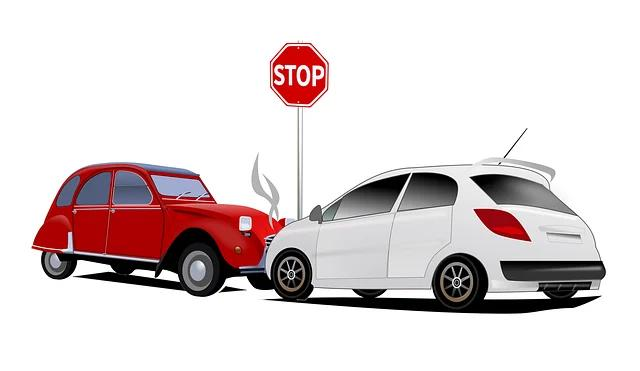
\includegraphics[width=\textwidth, height=2.9cm, keepaspectratio]{figures/tai-nan.jpg}

				\vspace{0.3em}

				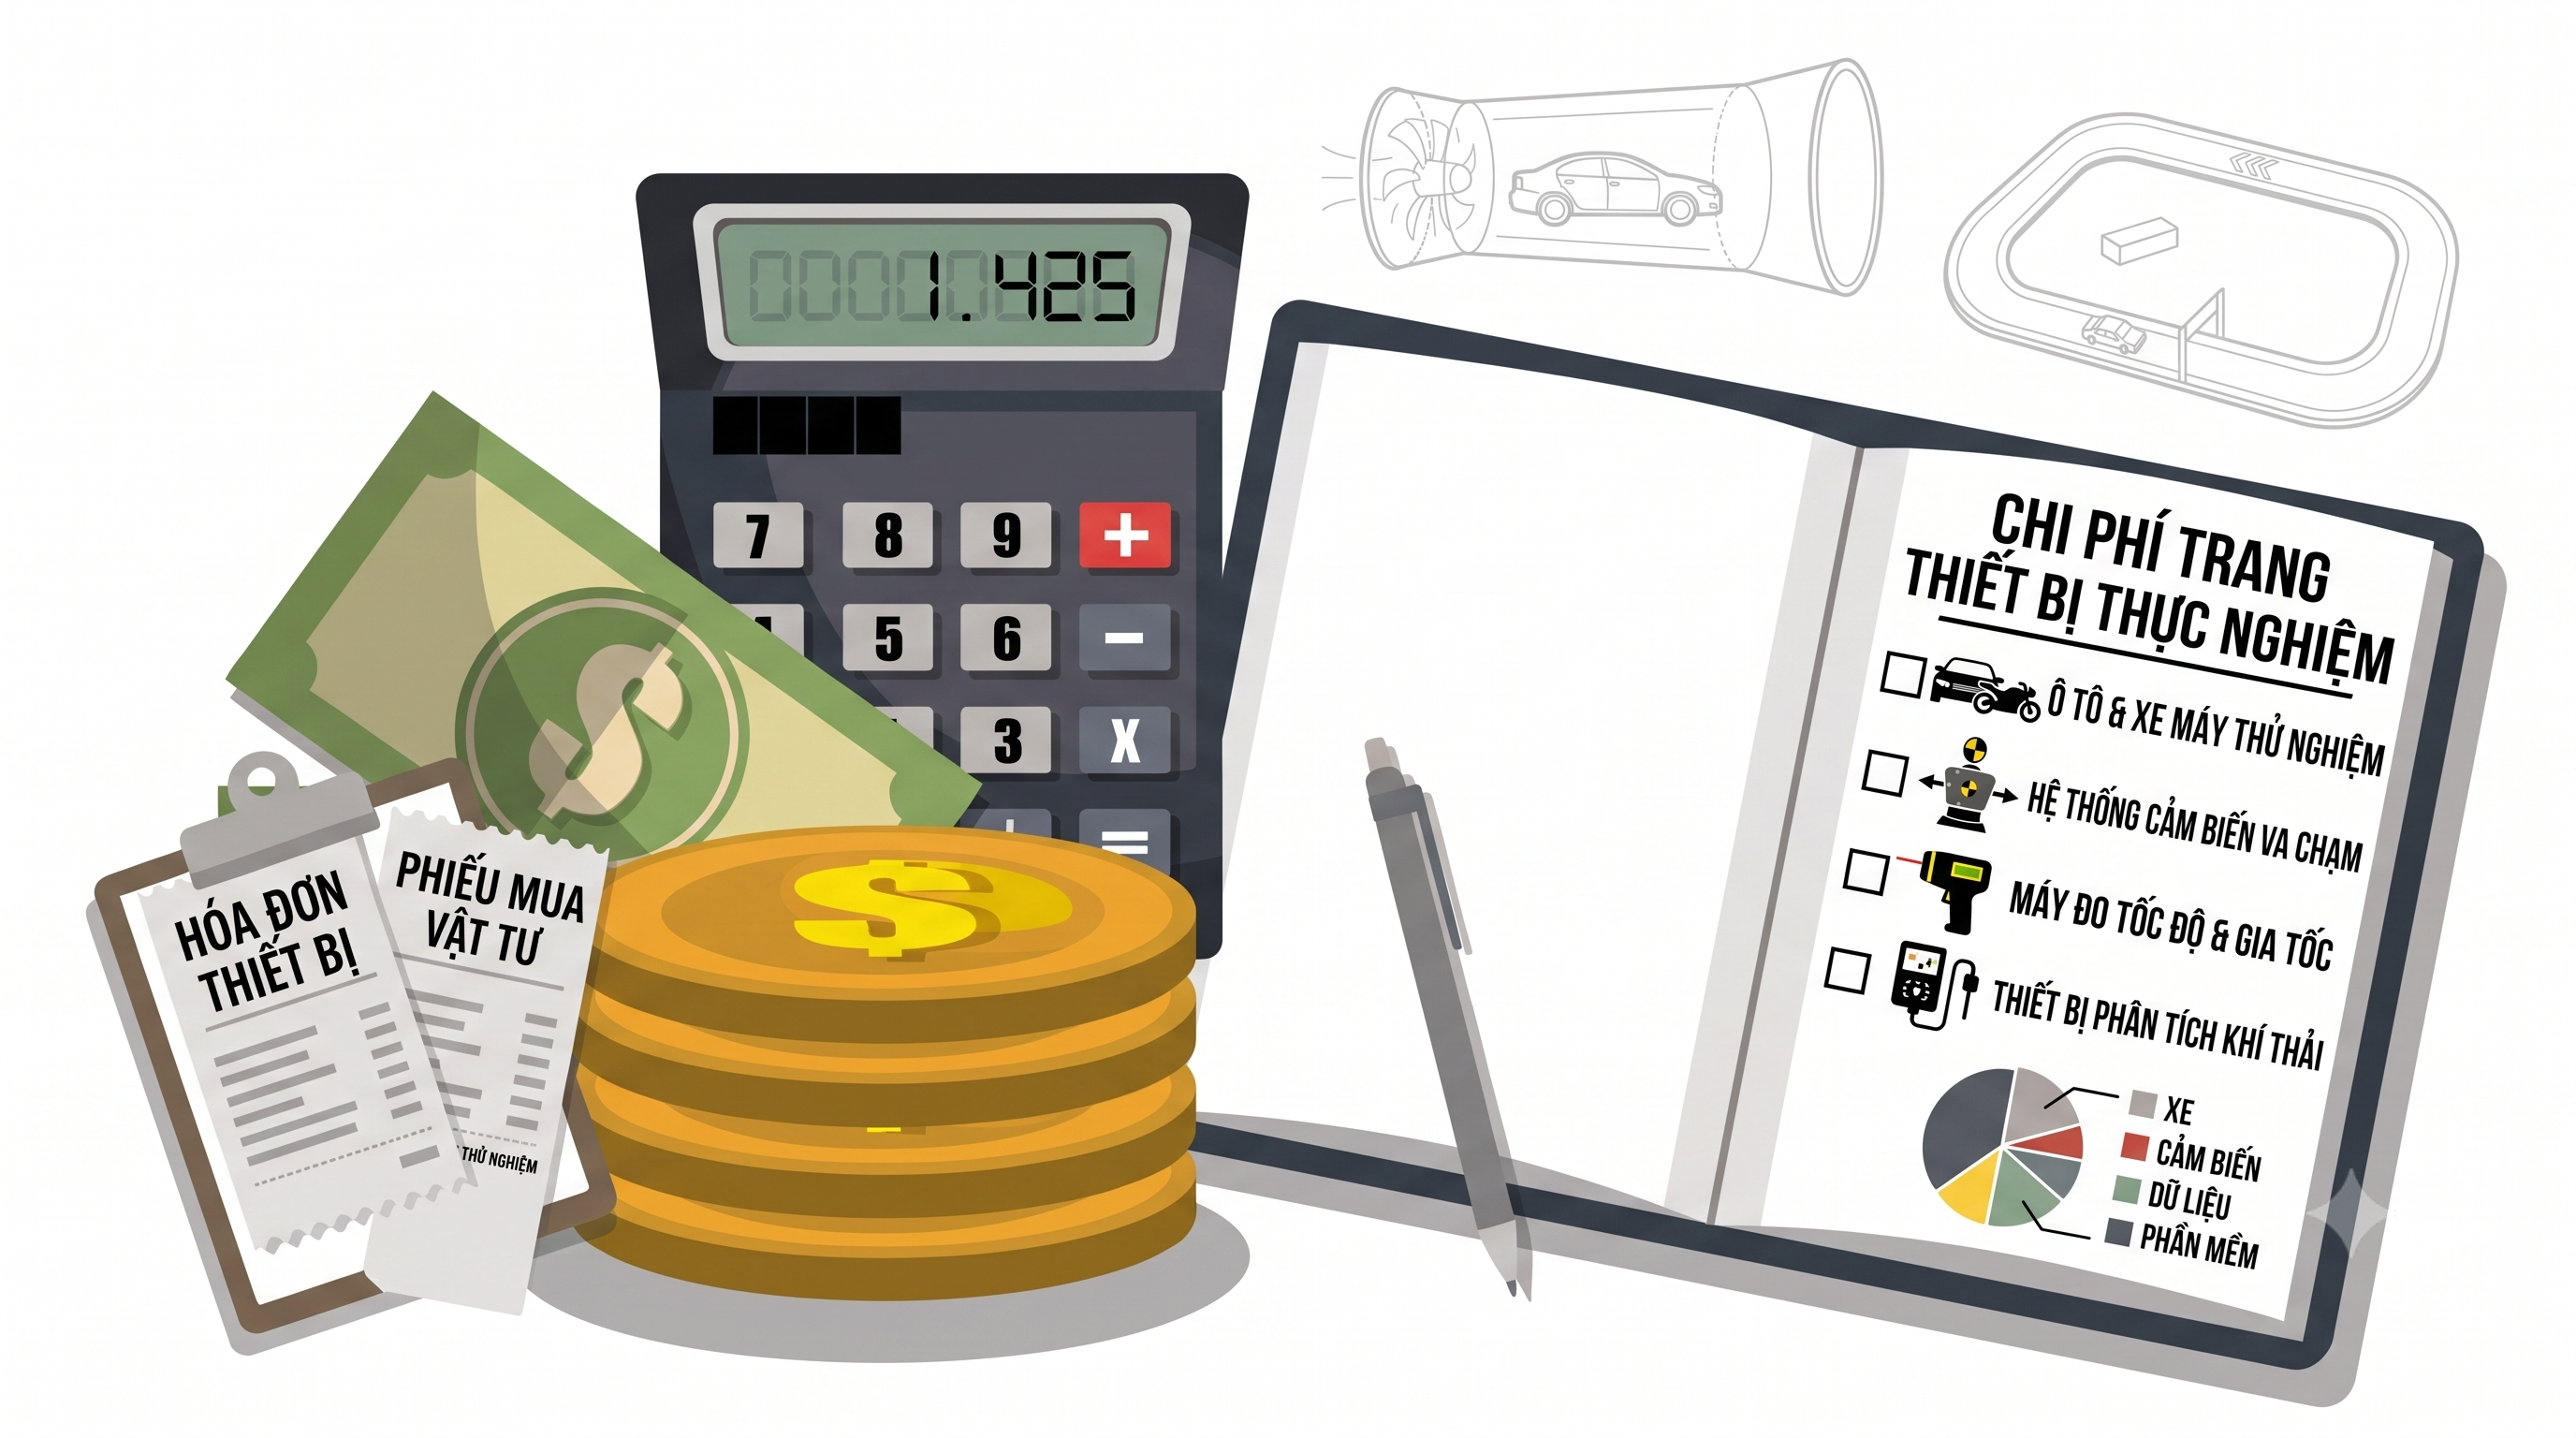
\includegraphics[width=\textwidth, height=2.9cm, keepaspectratio]{figures/chi-phi.png}
			\end{column}
		\end{columns}
	\end{frame}

	\begin{frame}{Hạn chế của SUMO 2D}
		\begin{columns}[T]
			\begin{column}{0.48\textwidth}
				\begin{block}{SUMO là gì?}
					\begin{itemize}
						\item Phần mềm mô phỏng giao thông vi mô \textbf{mã nguồn mở}
						\item Phổ biến trong nghiên cứu và học thuật
						\item Hỗ trợ mạng đường, làn xe, đèn tín hiệu, người đi bộ\ldots
					\end{itemize}
				\end{block}
			\end{column}
			\begin{column}{0.48\textwidth}
				\begin{alertblock}{Hạn chế}
					\begin{itemize}
						\item Góc nhìn 2D từ trên cao --- góc nhìn \textbf{người quản lý}
						\item Không tái hiện góc nhìn \textbf{người tham gia giao thông}
						\item Khó trình bày cho người không chuyên
						\item Không có tương tác trực tiếp với kịch bản
					\end{itemize}
				\end{alertblock}
			\end{column}
		\end{columns}

		\vspace{0.6em}
		$\Rightarrow$ Cần giải pháp hiển thị \textbf{3D tự động, tương tác được}, không đòi hỏi thao tác thủ công khi thay đổi kịch bản.
	\end{frame}

	\begin{frame}{Mục tiêu đề tài}
		\begin{columns}[T]
			\begin{column}{0.62\textwidth}
				\textbf{Chuỗi công nghệ:} SUMO $\;\rightarrow\;$ Python + TraCI $\;\rightarrow\;$ Unity (3D)

				\vspace{0.4em}
				\textbf{Bốn mục tiêu chính:}
				\begin{enumerate}\setlength{\itemsep}{0.2em}
					\item \textbf{Tự động dựng bản đồ 3D} từ dữ liệu SUMO / OpenStreetMap --- không cần thao tác thủ công
					\item \textbf{Thu thập trạng thái} phương tiện, đèn tín hiệu, người đi bộ theo từng bước mô phỏng qua TraCI
					\item \textbf{Hiển thị và cập nhật} đối tượng trong Unity theo thời gian thực, duy trì hiệu năng ổn định
					\item \textbf{Tương tác lái xe}: chiếm quyền điều khiển, xử lý va chạm, lưu \&{} phát lại kịch bản
				\end{enumerate}
			\end{column}
			\begin{column}{0.34\textwidth}
				\begin{minipage}[t][0.82\textheight][s]{\linewidth}
					\centering
					\vfill
					
\includegraphics[height=1.9cm, keepaspectratio]{figures/sumo-icon.png}
					\vfill
					
\includegraphics[height=1.9cm, keepaspectratio]{figures/python-icon.png}
					\vfill
					
\includegraphics[height=1.9cm, keepaspectratio]{figures/Unity-icon.png}
					\vfill
				\end{minipage}
			\end{column}
		\end{columns}
	\end{frame}

	% =================================================================
	% PHẦN 2: KIẾN TRÚC HỆ THỐNG
	% =================================================================
	\section{Kiến trúc hệ thống}

	\begin{frame}{Pipeline tổng quan}
		\begin{columns}[T]
			\begin{column}{0.44\textwidth}
				\begin{block}{Ba tầng kết nối}
					\begin{enumerate}
						\item \textbf{SUMO} --- chạy mô phỏng vi mô, quản lý xe, đèn, người đi bộ
						\item \textbf{Python + TraCI} --- đọc trạng thái từng bước, gửi sang Unity qua TCP/JSON
						\item \textbf{Unity} --- dựng cảnh 3D, hiển thị và xử lý tương tác
					\end{enumerate}
				\end{block}
			\end{column}
			\begin{column}{0.52\textwidth}
				\vspace{2.30em}
				\textbf{Luồng ngược:} vị trí xe người lái $\rightarrow$ Python $\rightarrow$ SUMO\\[0.3em]
				$\Rightarrow$ Hai tầng \textbf{tách biệt hoàn toàn} --- thay kịch bản SUMO, Unity tự cập nhật theo
			\end{column}
		\end{columns}
		\vspace{0.4em}
		\centering
		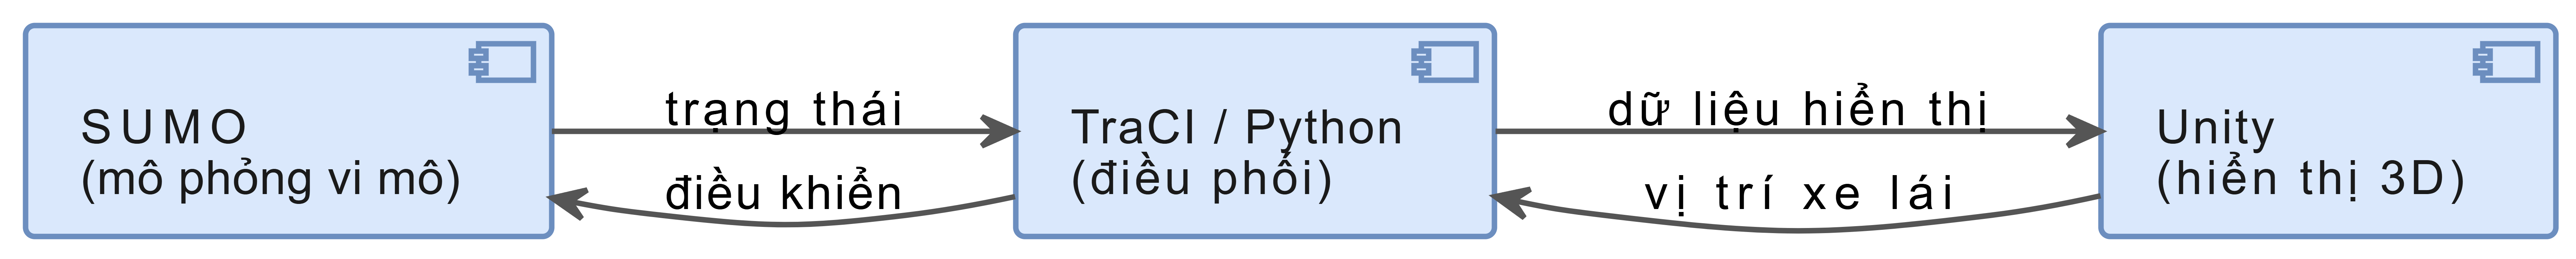
\includegraphics[width=0.9\textwidth, height=3.2cm, keepaspectratio]{../BaoCao_DATN/Hinhve/hinh3.1-kien-truc-tong-quat.png}
	\end{frame}

	% =================================================================
	% PHẦN 3: ĐÓNG GÓP KỸ THUẬT
	% =================================================================
	\section{Đóng góp kỹ thuật}

	\begin{frame}{Dựng bản đồ 3D chính xác}
		\begin{columns}[T]
			\begin{column}{0.58\textwidth}
				\textbf{Thách thức:} Dữ liệu SUMO chỉ là điểm tọa độ --- không có mesh 3D sẵn.

				\vspace{0.35em}
				\begin{block}{Đoạn đường --- dải lưới miter join}
					Tại khúc cua, mép làn lấy giao điểm hai đoạn kề (\emph{miter join}), khoảng lệch nhân $1/\cos\alpha$ để mép không bị bóp vào.
				\end{block}
				\vspace{0.3em}
				\begin{block}{Nút giao --- ear clipping + đùn khối}
					Tam giác hóa đa giác nút giao bằng \emph{ear clipping} (giữ hình lõm), đùn thành khối 3D. Tự chuyển sang bao lồi nếu đa giác tự cắt.
				\end{block}
			\end{column}
			\begin{column}{0.39\textwidth}
				\centering
				\resizebox{\linewidth}{!}{%
				\begin{tikzpicture}[>=Stealth]
					\coordinate (P0) at (0,0);
					\coordinate (P1) at (3,0);
					\coordinate (P2) at (5,1.5);
					\draw[dashed, gray] (P0) -- (P1) -- (P2);
					\foreach \p in {P0,P1,P2} \fill[gray] (\p) circle (1.5pt);
					\node[gray, below, font=\scriptsize] at (P0) {$P_0$};
					\node[gray, below, font=\scriptsize] at (P1) {$P_1$};
					\node[gray, right, font=\scriptsize] at (P2) {$P_2$};
					% mep trai/phai
					\draw[thick] (0,0.4) -- (2.86,0.4) -- (4.76,1.82);
					\draw[thick] (0,-0.4) -- (3.13,-0.4) -- (5.24,1.18);
					\draw (0,0.4) -- (0,-0.4);
					\draw (2.86,0.4) -- (3.13,-0.4);
					\draw (4.76,1.82) -- (5.24,1.18);
					% diagonal trong quad
					\draw[gray!60] (0,-0.4) -- (2.86,0.4);
					\node[above, font=\scriptsize] at (1.4,0.4) {mép trái};
					\node[below, font=\scriptsize] at (1.5,-0.4) {mép phải};
					% miter annotation
					\draw[->, red] (P1) -- ++(0.55,0.18) node[right, font=\scriptsize, red] {phân giác};
					\node[red, font=\scriptsize, align=center] at (3.5,-1.1) {khúc cua: nhân $1/\cos\alpha$\\để mesh không bị bóp};
					\draw[red, ->] (3.5,-0.8) -- (3.05,-0.3);
				\end{tikzpicture}}

				\vspace{0.5em}

				\begin{minipage}{0.44\linewidth}\centering
				\resizebox{\linewidth}{!}{%
				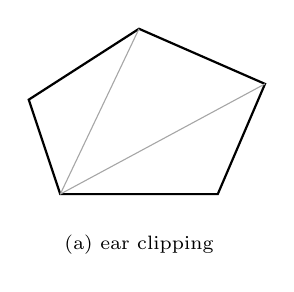
\begin{tikzpicture}
					\coordinate (A) at (0,0); \coordinate (B) at (2,0);
					\coordinate (C) at (2.6,1.4); \coordinate (D) at (1,2.1);
					\coordinate (E) at (-0.4,1.2);
					\draw[thick] (A)--(B)--(C)--(D)--(E)--cycle;
					\draw[gray!70] (A)--(C); \draw[gray!70] (A)--(D);
					\node[font=\scriptsize, below] at (1,-0.4) {(a) ear clipping};
				\end{tikzpicture}}
				\end{minipage}%
				\large$\;\rightarrow\;$%
				\begin{minipage}{0.44\linewidth}\centering
				\resizebox{\linewidth}{!}{%
				\begin{tikzpicture}
					\coordinate (A) at (0,0); \coordinate (B) at (2,0);
					\coordinate (C) at (2.6,1.4); \coordinate (D) at (1,2.1);
					\coordinate (E) at (-0.4,1.2);
					\draw[thick] (A)--(B)--(C)--(D)--(E)--cycle;
					\foreach \p in {A,B,C,D,E} \draw (\p) -- ($(\p)+(0,-0.6)$);
					\draw ($(A)+(0,-0.6)$)--($(B)+(0,-0.6)$)--($(C)+(0,-0.6)$)--($(D)+(0,-0.6)$)--($(E)+(0,-0.6)$)--cycle;
					\node[font=\scriptsize, below] at (1,-1.0) {(b) khối 3D};
				\end{tikzpicture}}
				\end{minipage}
			\end{column}
		\end{columns}
	\end{frame}

	\begin{frame}{Chiếm quyền \&{} lái xe tương tác}
		\begin{columns}[T]
			\begin{column}{0.58\textwidth}
				\begin{block}{Cơ chế chiếm quyền}
					\begin{itemize}\setlength{\itemsep}{0.15em}
						\item Người dùng chọn bất kỳ xe nào đang chạy, chiếm quyền tức thì
						\item Bật Rigidbody + Wheel Collider --- xe chuyển sang chuyển động vật lý
						\item Vị trí gửi ngược về SUMO --- xe xung quanh nhận biết và tránh
					\end{itemize}
				\end{block}

				\vspace{0.8em}
				\begin{alertblock}{Va chạm}
					\small Xe bị tông $\rightarrow$ trạng thái \textbf{xác xe}: nằm tại chỗ, gây ùn ứ --- tự dọn sau số bước định trước
				\end{alertblock}
			\end{column}
			\begin{column}{0.38\textwidth}
				\begin{minipage}[t][0.82\textheight][s]{\linewidth}
					\centering
					\vfill
					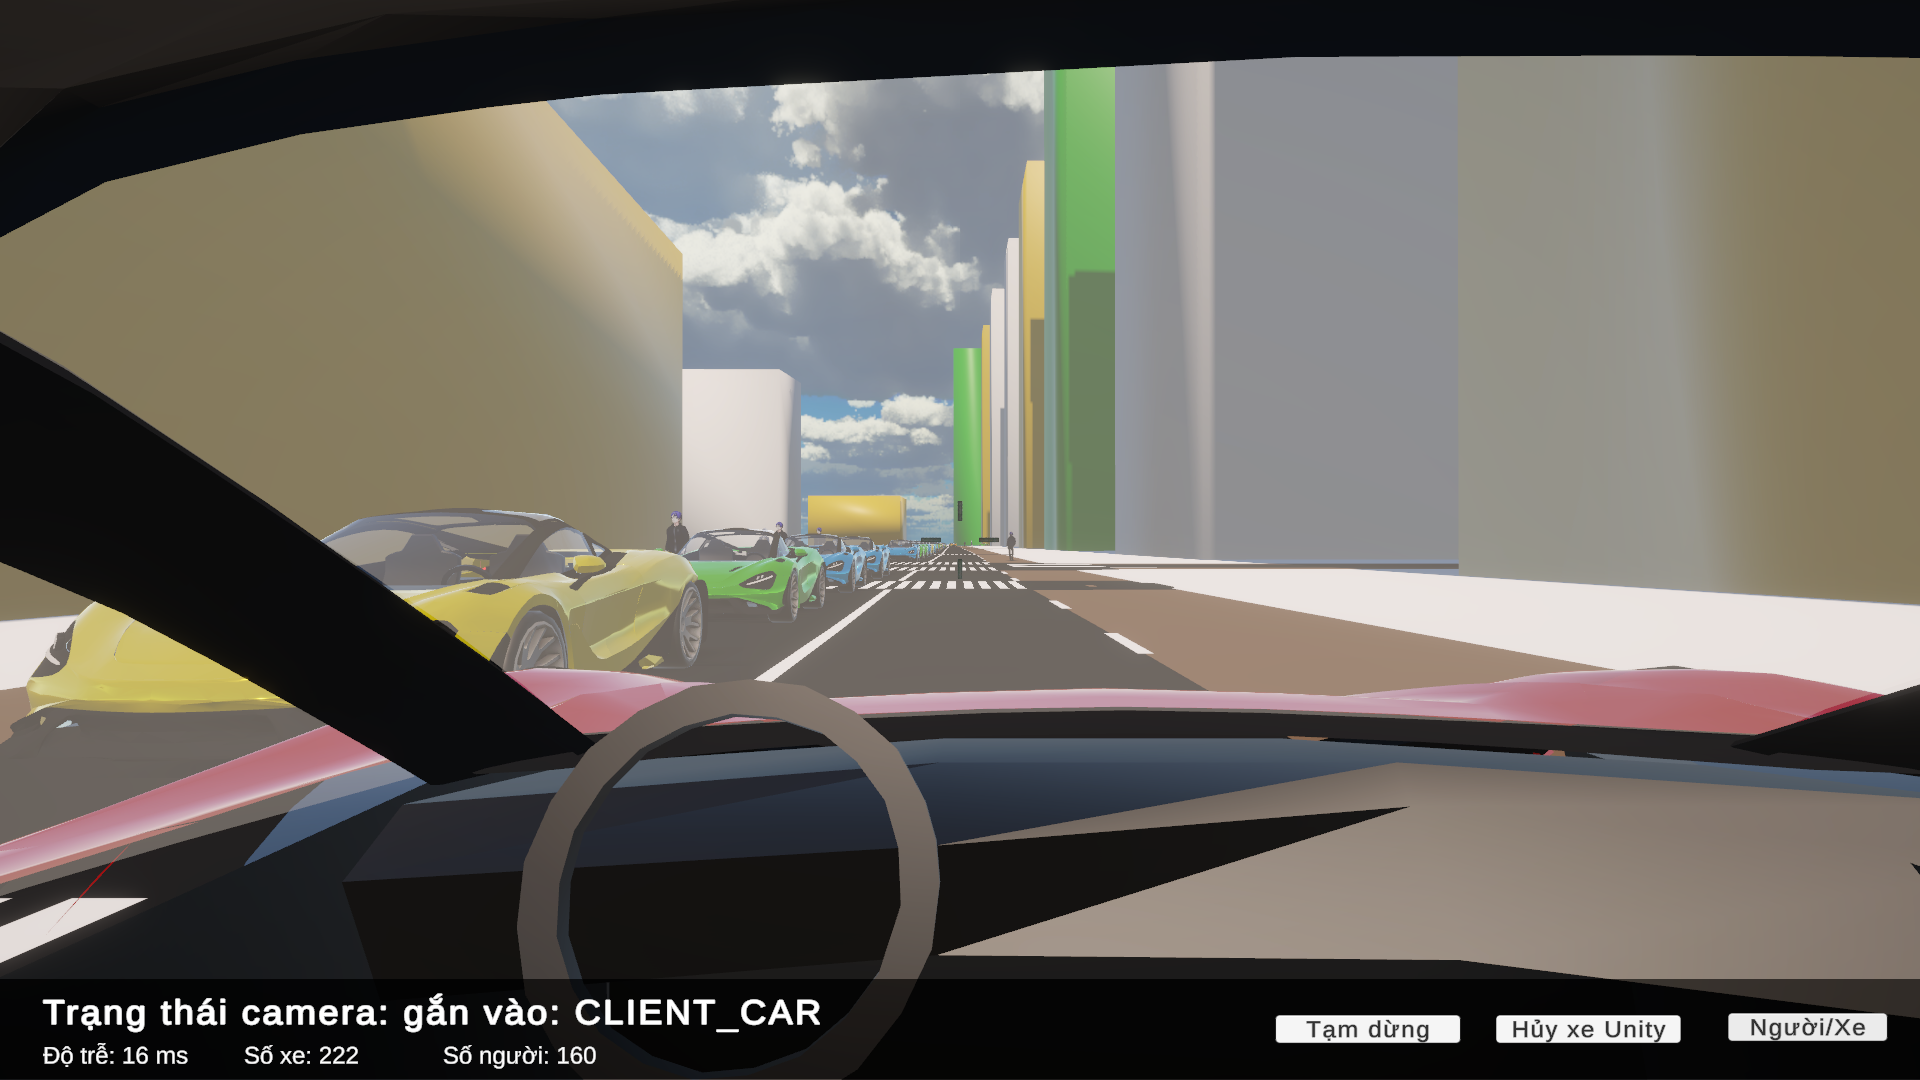
\includegraphics[width=\textwidth, keepaspectratio]{../BaoCao_DATN/Hinhve/hinh4.3.2b-goc-nhin-trong-xe.png}
					\vfill
					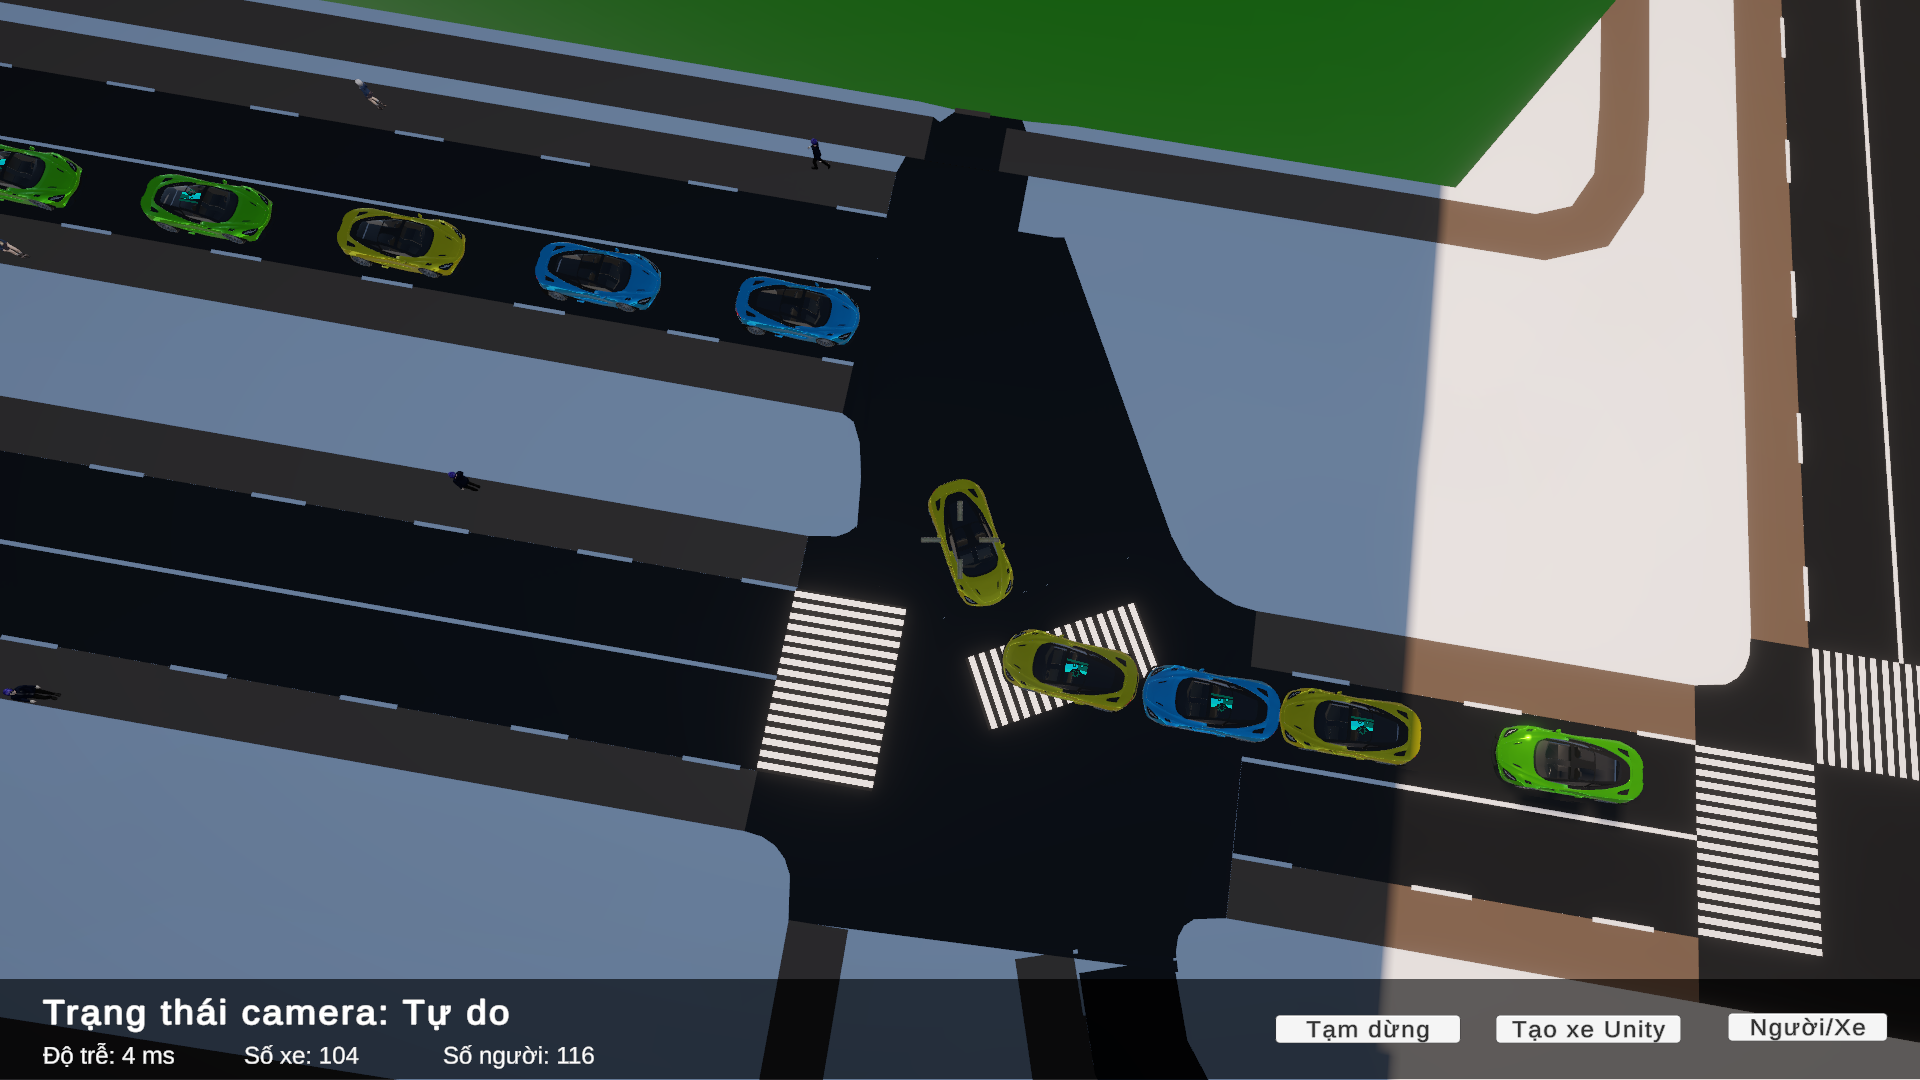
\includegraphics[width=\textwidth, keepaspectratio]{../BaoCao_DATN/Hinhve/hinh4.3.3-va-cham-gay-un-tac.png}
					\vfill
				\end{minipage}
			\end{column}
		\end{columns}
	\end{frame}

	\begin{frame}{Lưu \&{} phát lại kịch bản}
		\begin{minipage}[t][0.82\textheight][s]{\textwidth}
			% --- Phần trên: nội dung ---
			\begin{columns}[T]
				\begin{column}{0.44\textwidth}
					\begin{block}{Lưu trữ theo phiên}
						\begin{itemize}\setlength{\itemsep}{0.1em}
							\item Mỗi lần chạy gom vào một thư mục theo tên bản đồ và thời điểm
							\item Chuỗi trạng thái ghi luồng --- không giữ toàn bộ trong RAM
							\item Kèm dữ liệu mạng đường, nhật ký hành trình, bản tóm tắt
						\end{itemize}
					\end{block}
				\end{column}
				\begin{column}{0.52\textwidth}
					\vspace{0.72em}
					\begin{itemize}\setlength{\itemsep}{0.2em}
						\item Đọc lại chuỗi trạng thái, tái hiện trong Unity
						\item \textbf{Không cần khởi động lại SUMO} --- thuận tiện cho phân tích và trình bày kết quả
					\end{itemize}
				\end{column}
			\end{columns}
			\vfill
			% --- Phần dưới: ảnh ---
			\hfill
			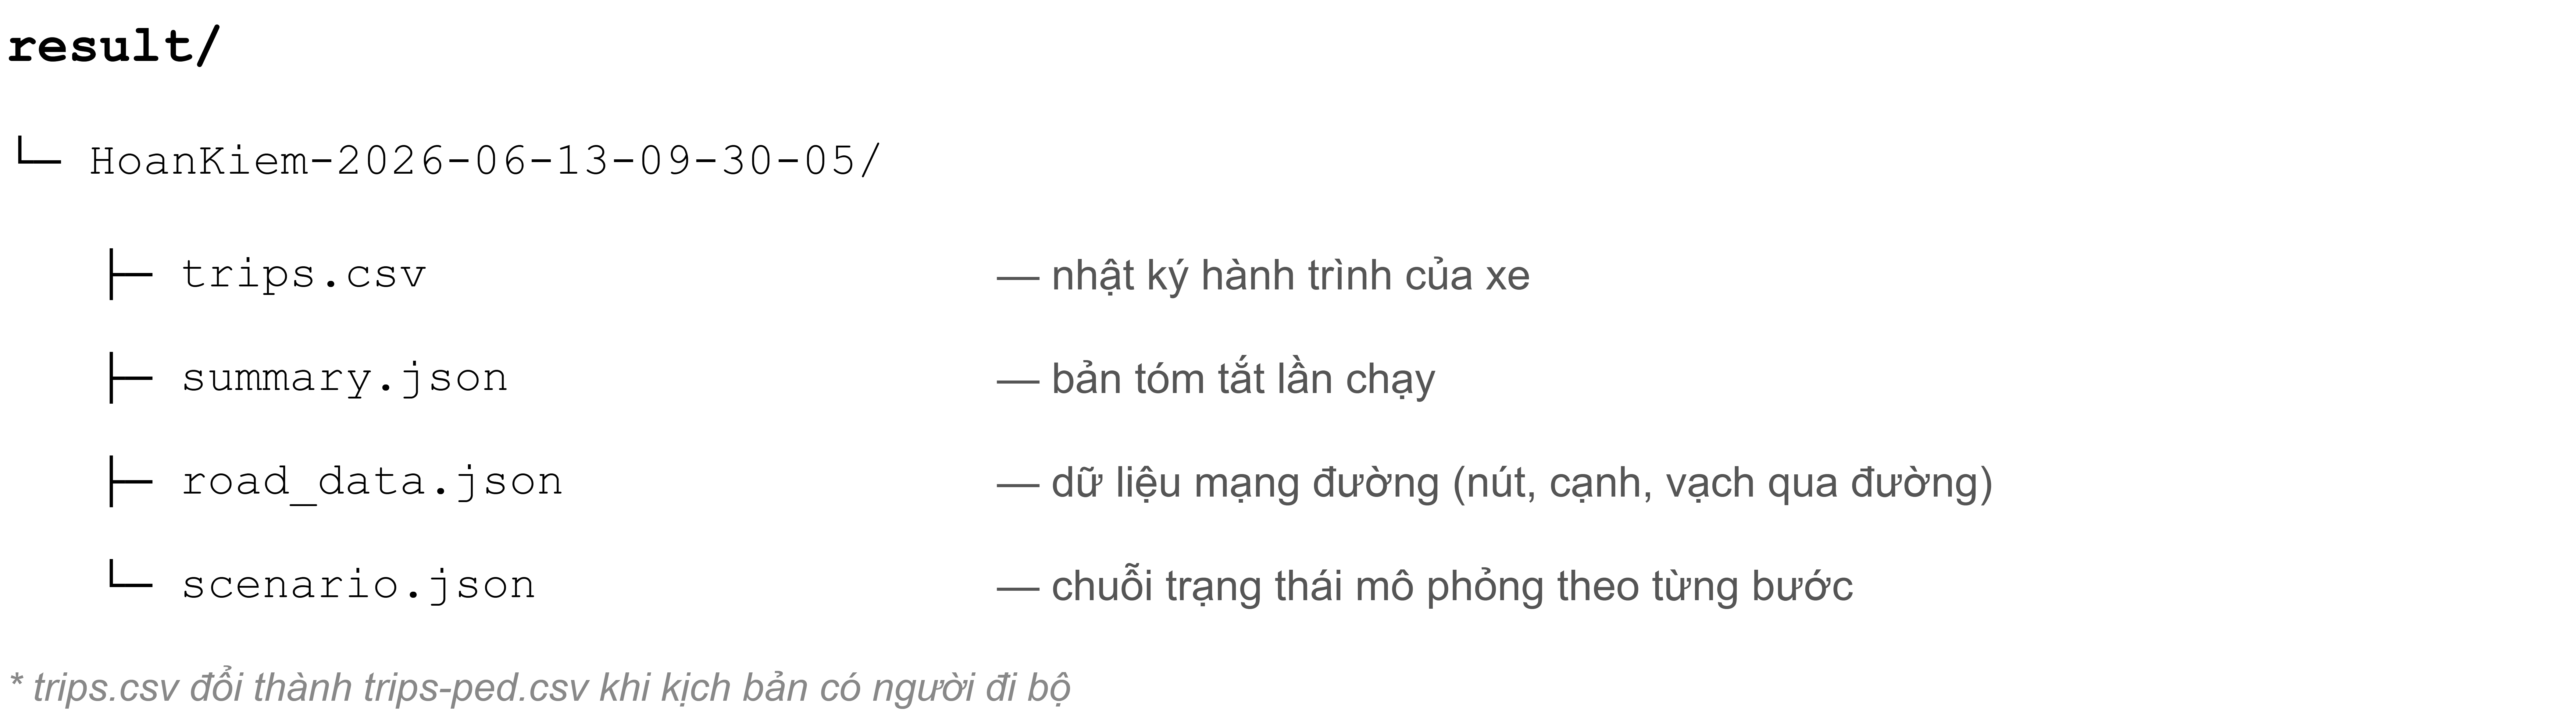
\includegraphics[width=0.80\textwidth, height=0.41\textheight, keepaspectratio]{../BaoCao_DATN/Hinhve/hinh4.2.6-cau-truc-thu-muc-phien.png}
			\vfill
		\end{minipage}
	\end{frame}

	\begin{frame}{Tối ưu hiệu năng hiển thị}
		\begin{columns}[T]
			\begin{column}{0.48\textwidth}
				\begin{enumerate}\setlength{\itemsep}{0.3em}
					\item \textbf{Tái sử dụng đối tượng (Object Pool)}\\ Xe rời mạng không bị hủy mà được thu hồi --- giảm chi phí tạo/hủy liên tục
					\item \textbf{Lọc theo vùng quan sát}\\ Chỉ hiển thị xe trong tầm camera, tạm ẩn xe ngoài tầm --- giảm số lệnh vẽ
					\item \textbf{Nội suy chuyển động}\\ Vị trí xe được nội suy giữa hai bước SUMO --- chuyển động mượt dù SUMO chỉ cập nhật mỗi 0,1 giây
				\end{enumerate}
			\end{column}
			\begin{column}{0.48\textwidth}
				\begin{minipage}[c][0.82\textheight][c]{\linewidth}
					\centering
					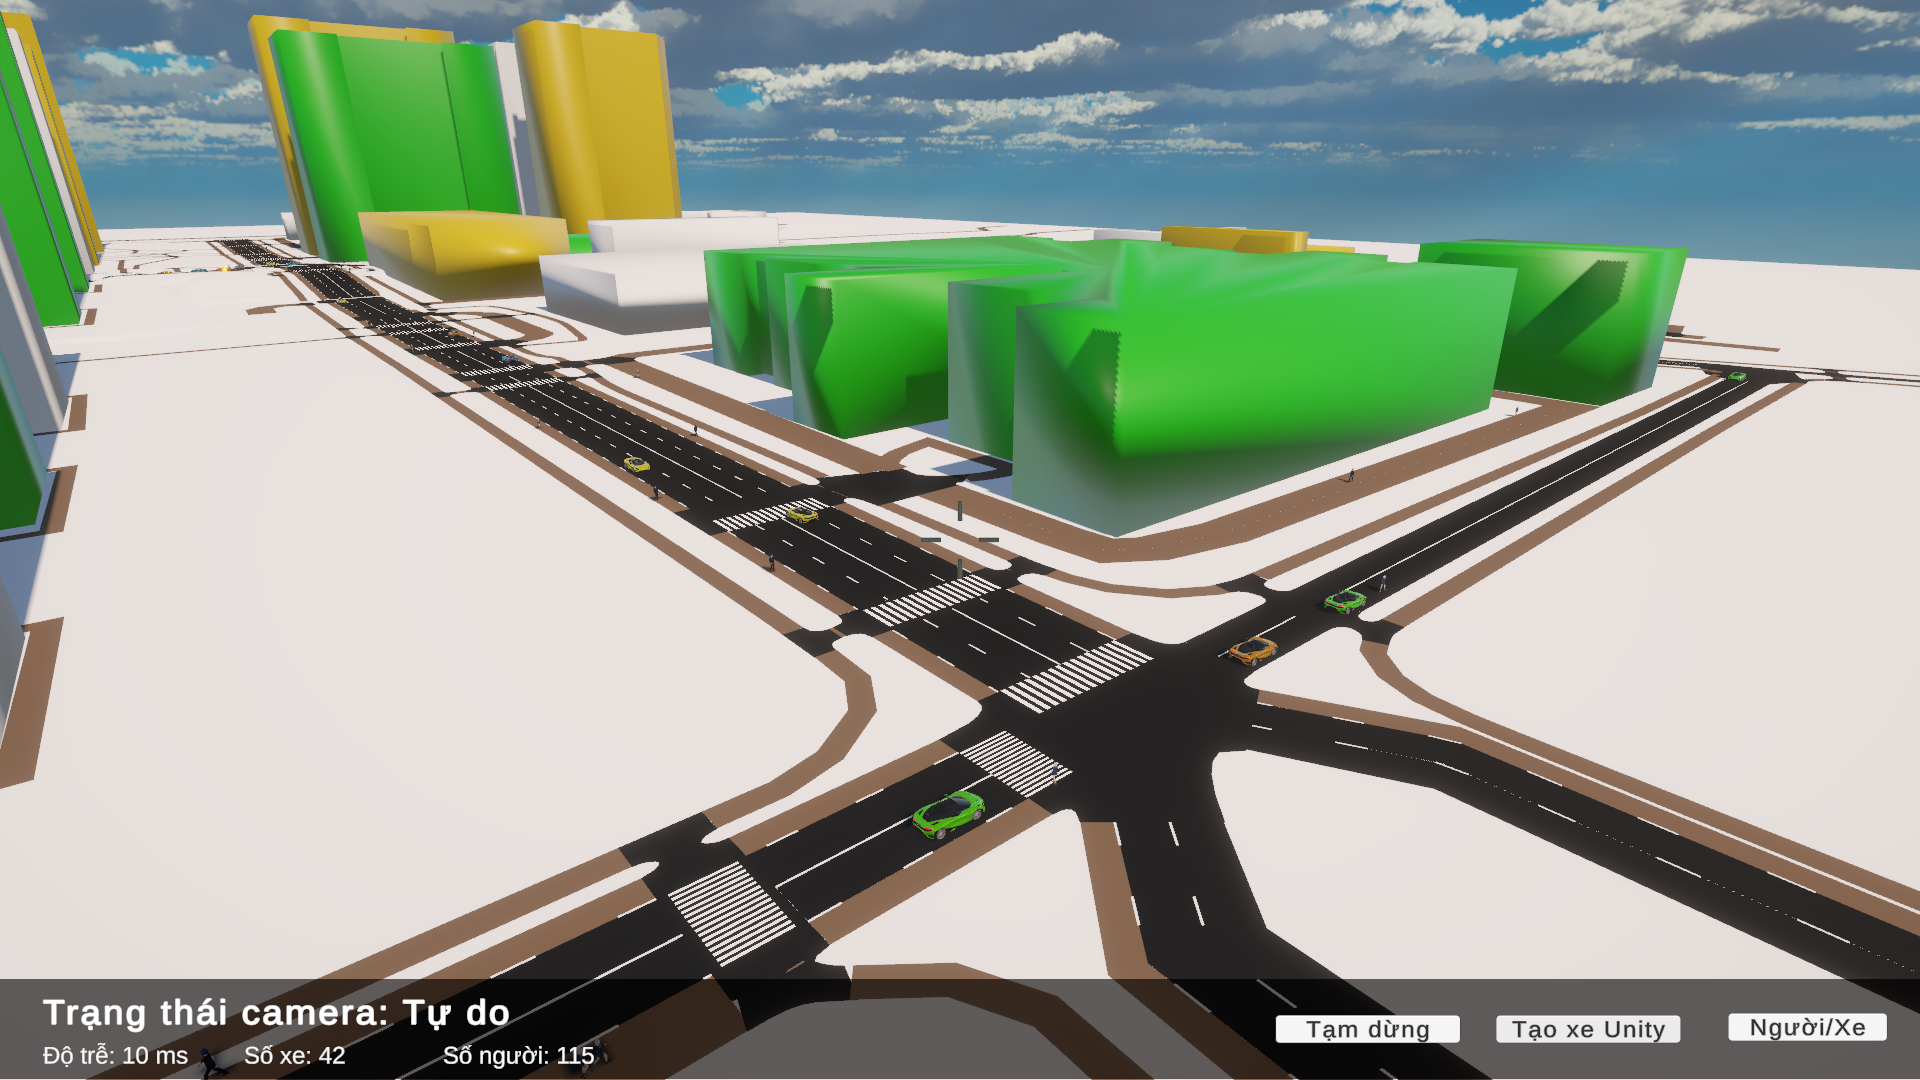
\includegraphics[width=\textwidth, keepaspectratio]{../BaoCao_DATN/Hinhve/hinh4.3.1-anh-goc-nhin-3d-tu-tren-cao.png}
				\end{minipage}
			\end{column}
		\end{columns}
	\end{frame}

	% =================================================================
	% PHẦN 4: KẾT QUẢ
	% =================================================================
	\section{Kết quả}

	\begin{frame}{Kiểm thử}
		\begin{columns}[T]
			\begin{column}{0.58\textwidth}
				\small
				\begin{tabular}{|p{0.08\linewidth}|p{0.52\linewidth}|c|}
					\hline
					\textbf{TC} & \textbf{Nội dung} & \textbf{Kết quả} \\
					\hline
					TC01 & Nhận dữ liệu mạng đường, dựng cảnh & \textcolor{green!60!black}{\textbf{Đạt}} \\ \hline
					TC02 & Hiển thị trạng thái đèn tín hiệu & \textcolor{green!60!black}{\textbf{Đạt}} \\ \hline
					TC03 & Chiếm quyền và lái xe tương tác & \textcolor{green!60!black}{\textbf{Đạt}} \\ \hline
					TC04 & Va chạm sinh xác xe, tự dọn & \textcolor{green!60!black}{\textbf{Đạt}} \\ \hline
				\end{tabular}

				\vspace{0.6em}
				$\Rightarrow$ Tất cả 4 ca kiểm thử \textbf{đều đạt}. Hiện tượng duy nhất: lệch đồng bộ nhẹ khi tốc độ mô phỏng quá cao so với phần cứng.
			\end{column}
			\begin{column}{0.38\textwidth}
				\begin{minipage}[c][0.82\textheight][c]{\linewidth}
					\centering
					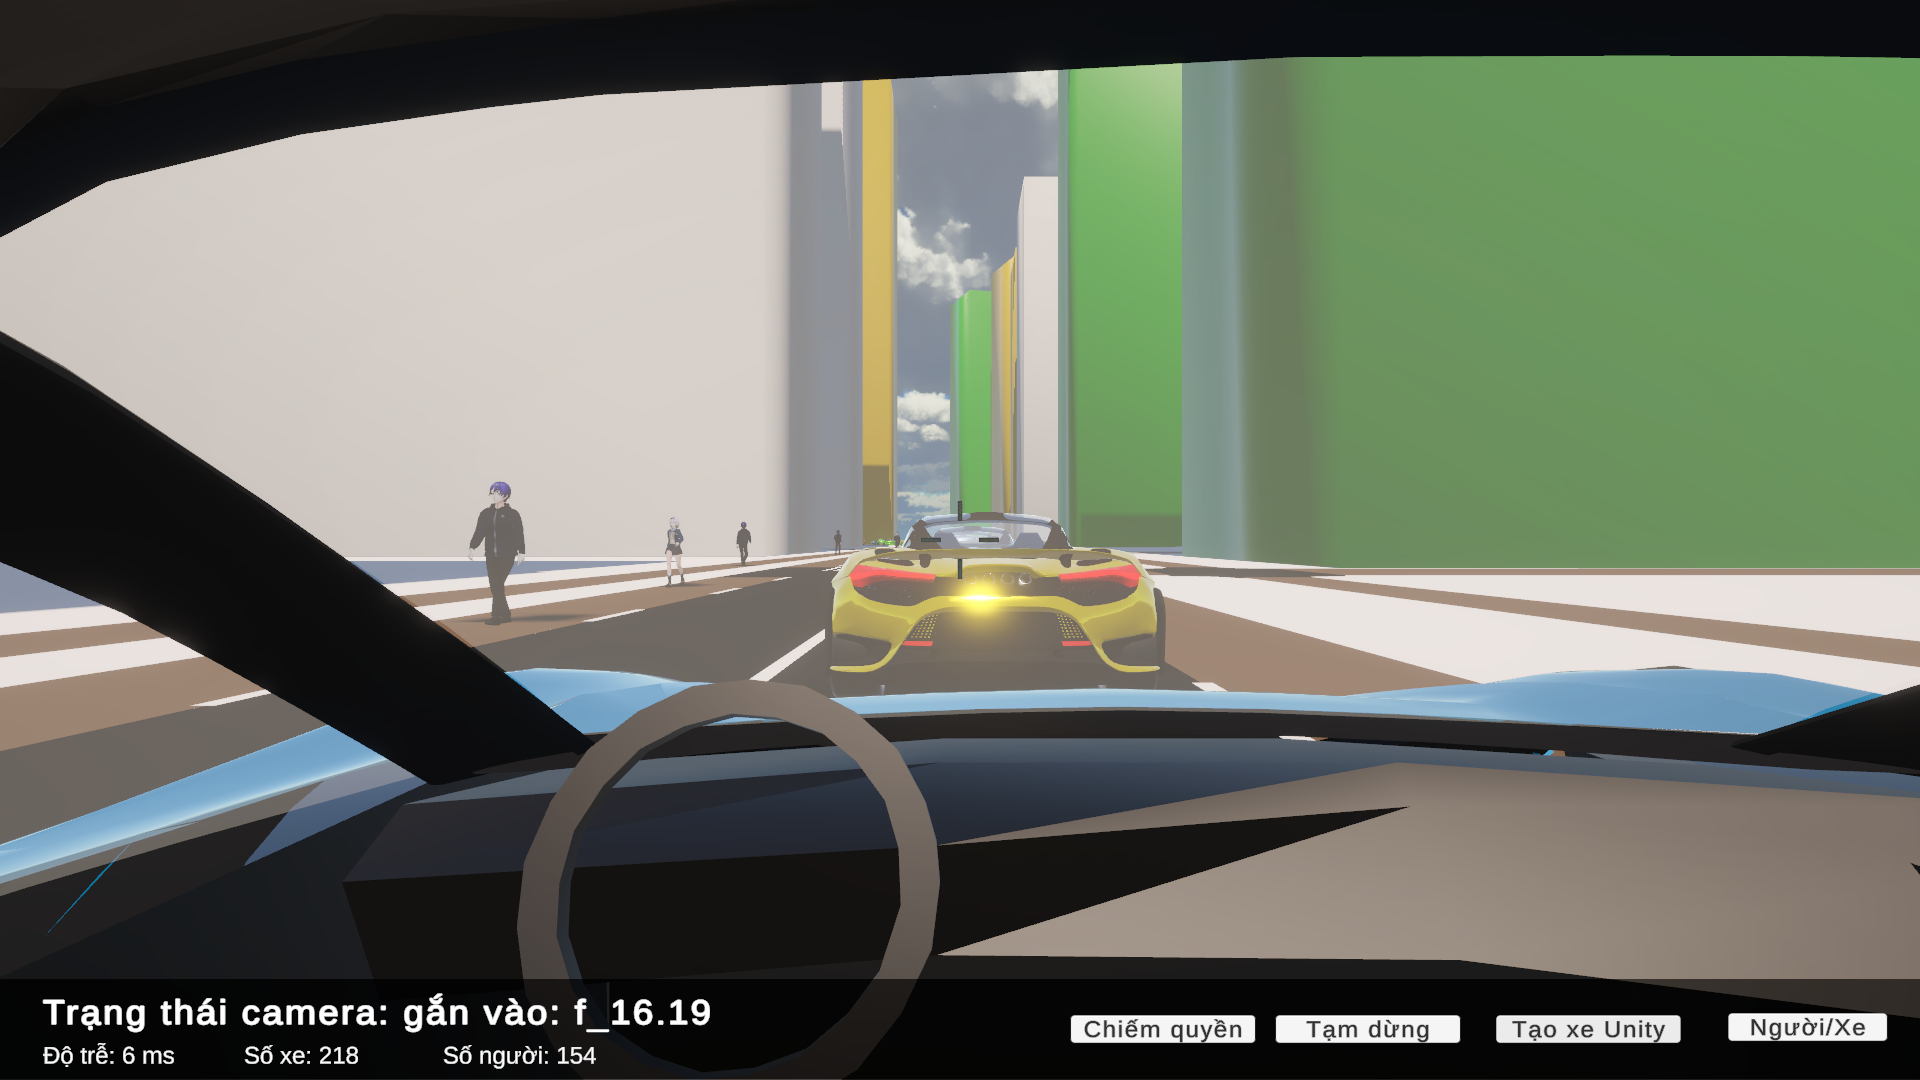
\includegraphics[width=\textwidth, keepaspectratio]{../BaoCao_DATN/Hinhve/hinh4.3.2a-goc-nhin-cua-1-xe-tu-hanh-boi-may-chu.png}
				\end{minipage}
			\end{column}
		\end{columns}
	\end{frame}

	\begin{frame}{Đánh giá hiệu năng}
		\textbf{Máy bàn} (i5-14400F, RTX 4060) --- giới hạn Unity 120 FPS:

		\vspace{0.3em}
		{\small
		\begin{tabular}{|p{0.34\linewidth}|c|c|c|c|}
			\hline
			\textbf{Kịch bản} & \textbf{Đối tượng} & \textbf{FPS TB} & \textbf{FPS min} & \textbf{Trễ (ms)} \\
			\hline
			Mê cung nhỏ (32$\times$32)   & 100 xe + 100 người & 119.5 & 52.9 & 6.2 \\ \hline
			Mê cung vừa (64$\times$64)   & 100 xe + 100 người & 112.1 & 40.6 & 8.3 \\ \hline
			Mê cung lớn (128$\times$128) & 100 xe + 100 người & 100.1 & 11.9 & 13.0 \\ \hline
			Bản đồ OSM thực tế           &  50 xe + 50 người  & \textbf{119.8} & 93.3 & \textbf{6.2} \\ \hline
		\end{tabular}}

		\vspace{0.5em}
		\textbf{Laptop phổ thông} (i5-1240P, MX570) --- bản đồ OSM:

		\vspace{0.3em}
		{\small
		\begin{tabular}{|p{0.34\linewidth}|c|c|c|c|}
			\hline
			\textbf{Kịch bản} & \textbf{Đối tượng} & \textbf{FPS TB} & \textbf{FPS min} & \textbf{Trễ (ms)} \\
			\hline
			Bản đồ OSM thực tế & 50 xe + 50 người & \textbf{81.5} & 40.8 & 11.8 \\ \hline
		\end{tabular}}

		\vspace{0.4em}
		$\Rightarrow$ Hệ thống vận hành ổn định trên phần cứng thông thường, không đòi hỏi thiết bị chuyên dụng.
	\end{frame}

	% =================================================================
	% PHẦN 5: KẾT LUẬN
	% =================================================================
	\section{Kết luận}

	\begin{frame}{Kết luận}
		\begin{block}{Kết quả đạt được}
			\begin{itemize}\setlength{\itemsep}{0.3em}
				\item \textbf{Tự động dựng bản đồ 3D} từ bất kỳ kịch bản SUMO / OpenStreetMap, không cần thao tác thủ công
				\item \textbf{Hiển thị đa đối tượng} --- xe, đèn tín hiệu, người đi bộ theo thời gian thực, chuyển động mượt
				\item \textbf{Tương tác lái xe} --- chiếm quyền, lái bằng vật lý, xử lý va chạm, lưu \&{} phát lại kịch bản
				\item \textbf{Hiệu năng ổn định} --- OSM đạt 119,8 FPS (máy bàn), 81,5 FPS (laptop phổ thông)
			\end{itemize}
		\end{block}

		\vspace{0.8em}
		$\Rightarrow$ Hệ thống cho phép người dùng \textbf{thực sự tham gia vào dòng giao thông} thay vì chỉ quan sát từ góc nhìn 2D từ trên cao.
	\end{frame}

	\begin{frame}{Hướng phát triển}
		\begin{columns}[T]
			\begin{column}{0.64\textwidth}
				\small
				\begin{itemize}\setlength{\itemsep}{0.2em}
					\item \textbf{Hoàn thiện tương tác:} tái nhập làn tự nhiên khi trả quyền, hỗ trợ va chạm người--xe, đa người dùng cùng phiên
					\item \textbf{Mở rộng phương tiện:} thêm xe máy, xe tải, xe buýt với đặc tính di chuyển riêng
					\item \textbf{Tối ưu truyền thông:} giao thức nhị phân thay JSON, mã hóa sai phân, lọc theo vùng quan sát
					\item \textbf{Thời tiết \&{} môi trường:} mưa, gió, tuyết ảnh hưởng hành vi xe; thêm tòa nhà chi tiết, cây cối, biển báo, đèn đường
					\item Hướng tới \textbf{tựa game đô thị} với đồ họa chất lượng cao --- ưu tiên tái hiện các thành phố Việt Nam
				\end{itemize}
			\end{column}
			\begin{column}{0.32\textwidth}
				\begin{minipage}[c][0.82\textheight][c]{\linewidth}
					\centering
					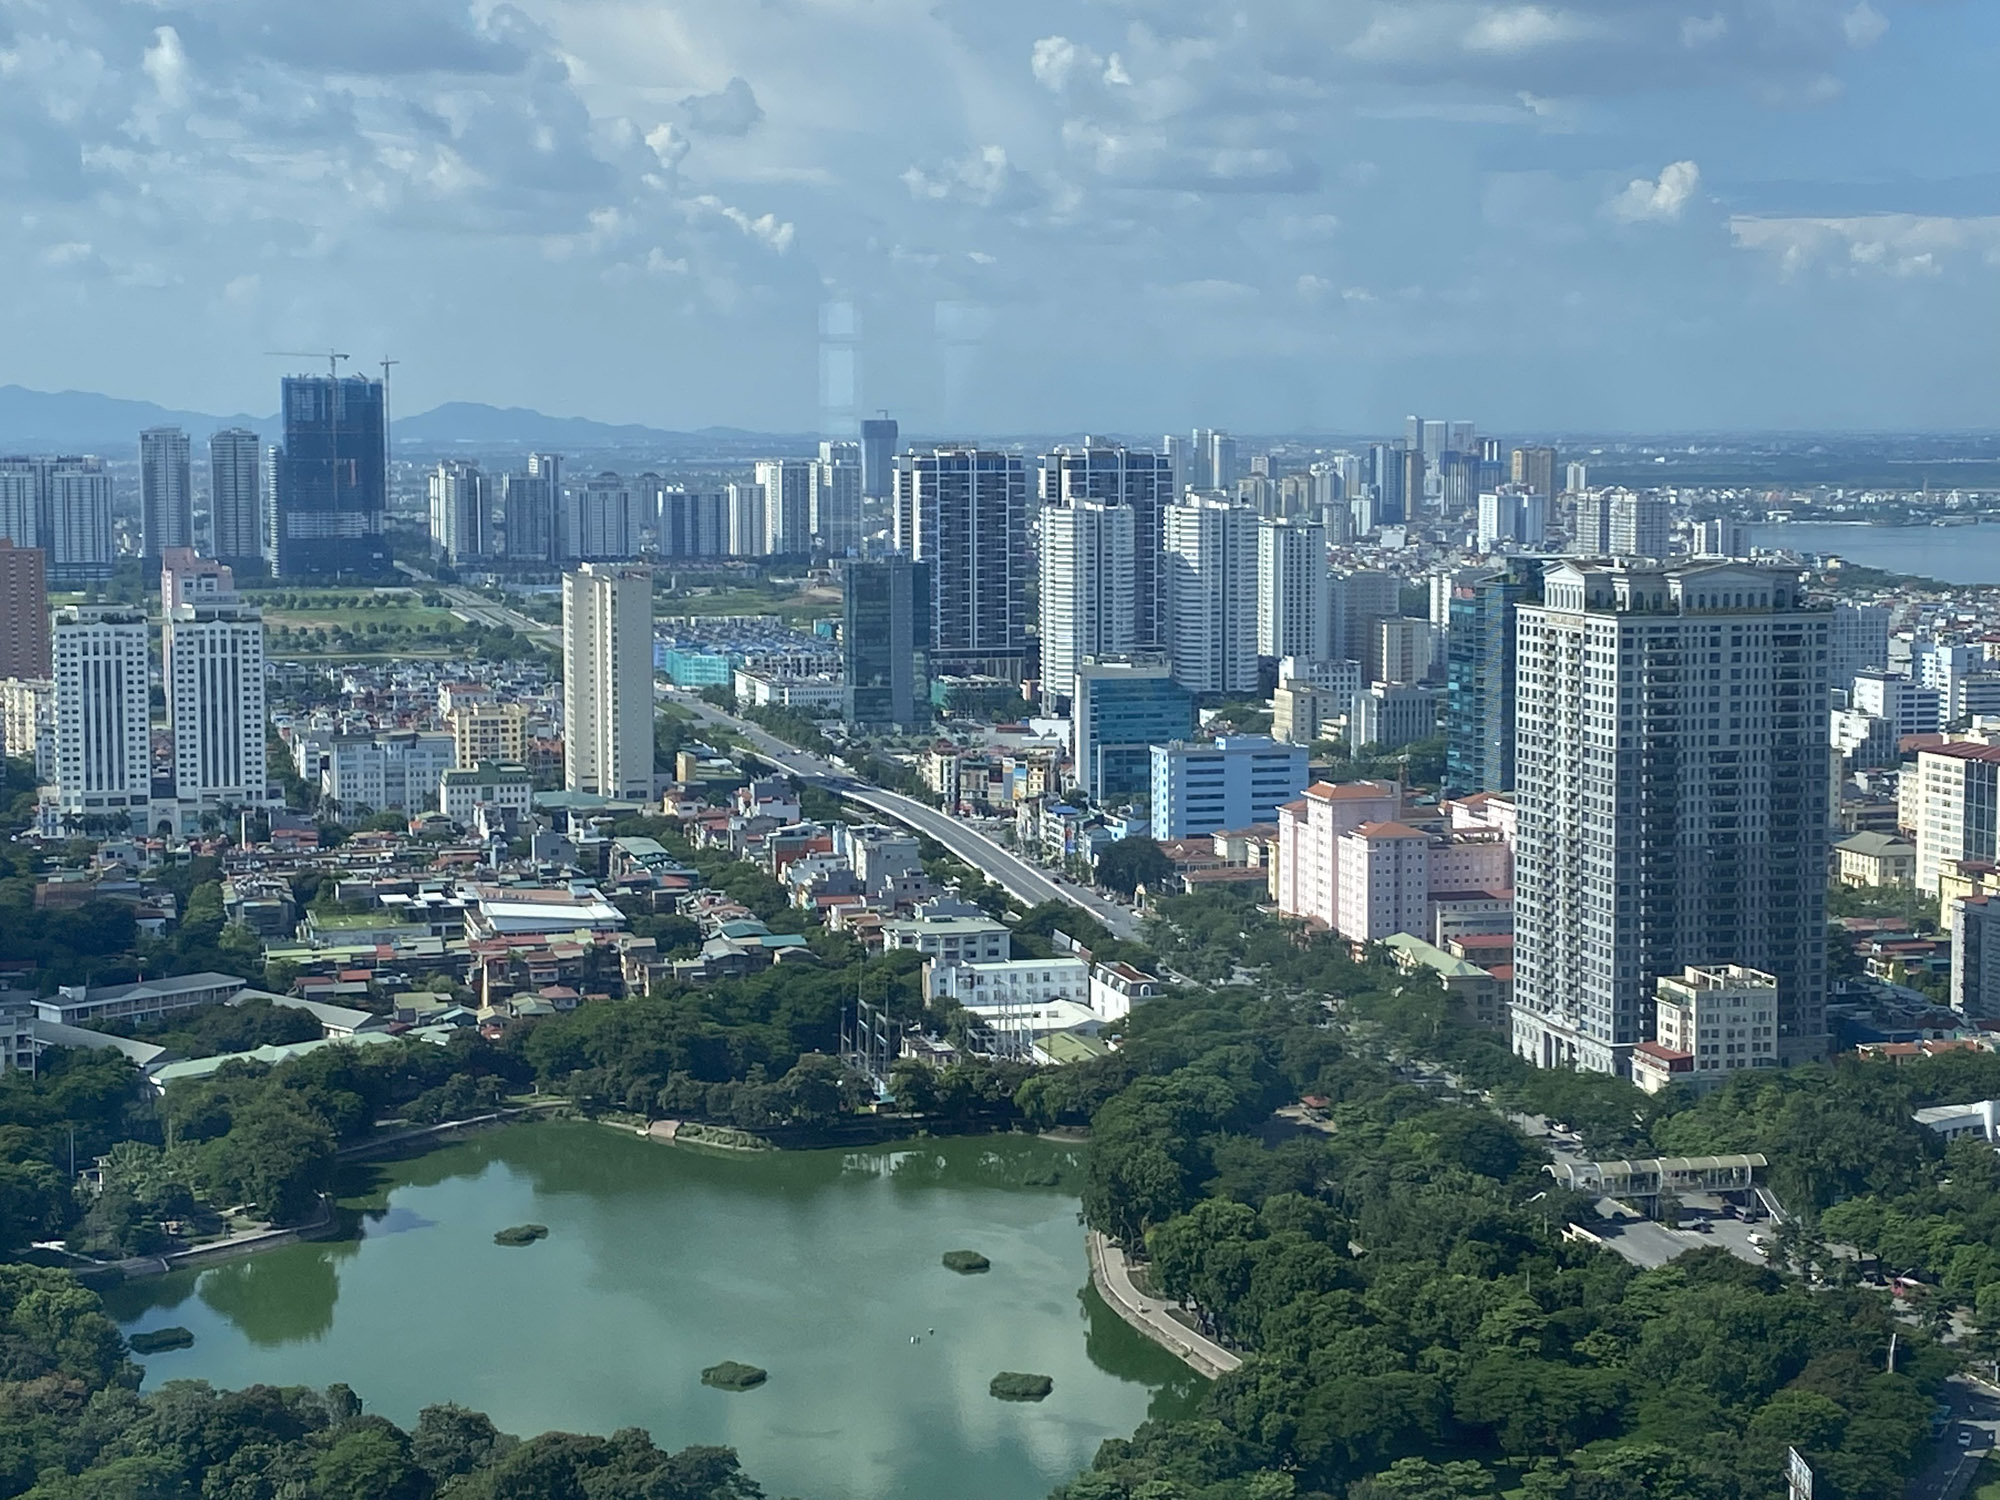
\includegraphics[width=\textwidth, keepaspectratio]{figures/real-city.png}
				\end{minipage}
			\end{column}
		\end{columns}
	\end{frame}

	% =================================================================
	% KẾT THÚC
	% =================================================================
	\hustthankyou

\end{document}